\documentclass[a4paper]{article}
% Template from: https://github.com/johnjohnlin/oreilly_cover

\usepackage{lmodern}         % for the looks
\usepackage[T1]{fontenc}     % to hypenate accented characters correctly
\usepackage[utf8]{inputenc}  % just in case we go for non-ascii
\usepackage{tikz}            % the graphics
\usepackage{textcomp}        % for \textregistered

\begin{document}
\thispagestyle{empty}

\begin{tikzpicture}[remember picture,overlay]

\node [align=center] at (current page.north) % upper
      {\begin{tikzpicture}[remember picture, overlay]
	  \fill[fill=blue!30] (-10,0) rectangle (10,-0.5);
	  \node[anchor=north] at (0,-0.5) {\Large\textit{Descriptive Development}};
      \end{tikzpicture}};
      
\node [yshift=-5cm] at (current page.center) % title
{\begin{tikzpicture}[remember picture, overlay]
		\fill[fill=blue!30] (-10,-5) rectangle (10 ,1);
		\node[align=center] at (0,-2)
		{\resizebox{1.57\linewidth}{!}{\Huge\textbf{Project Design Builder}}};
		\node[anchor=east,align=right] at (10,-5.5) {\Huge\color{black}\textit{Dynamic Complex Generation}};
\end{tikzpicture}};

\node [align=center] at (current page.center) % dragon
      {\begin{tikzpicture}[remember picture, overlay]
          \node[anchor=center,align=center] at (0,4)
               {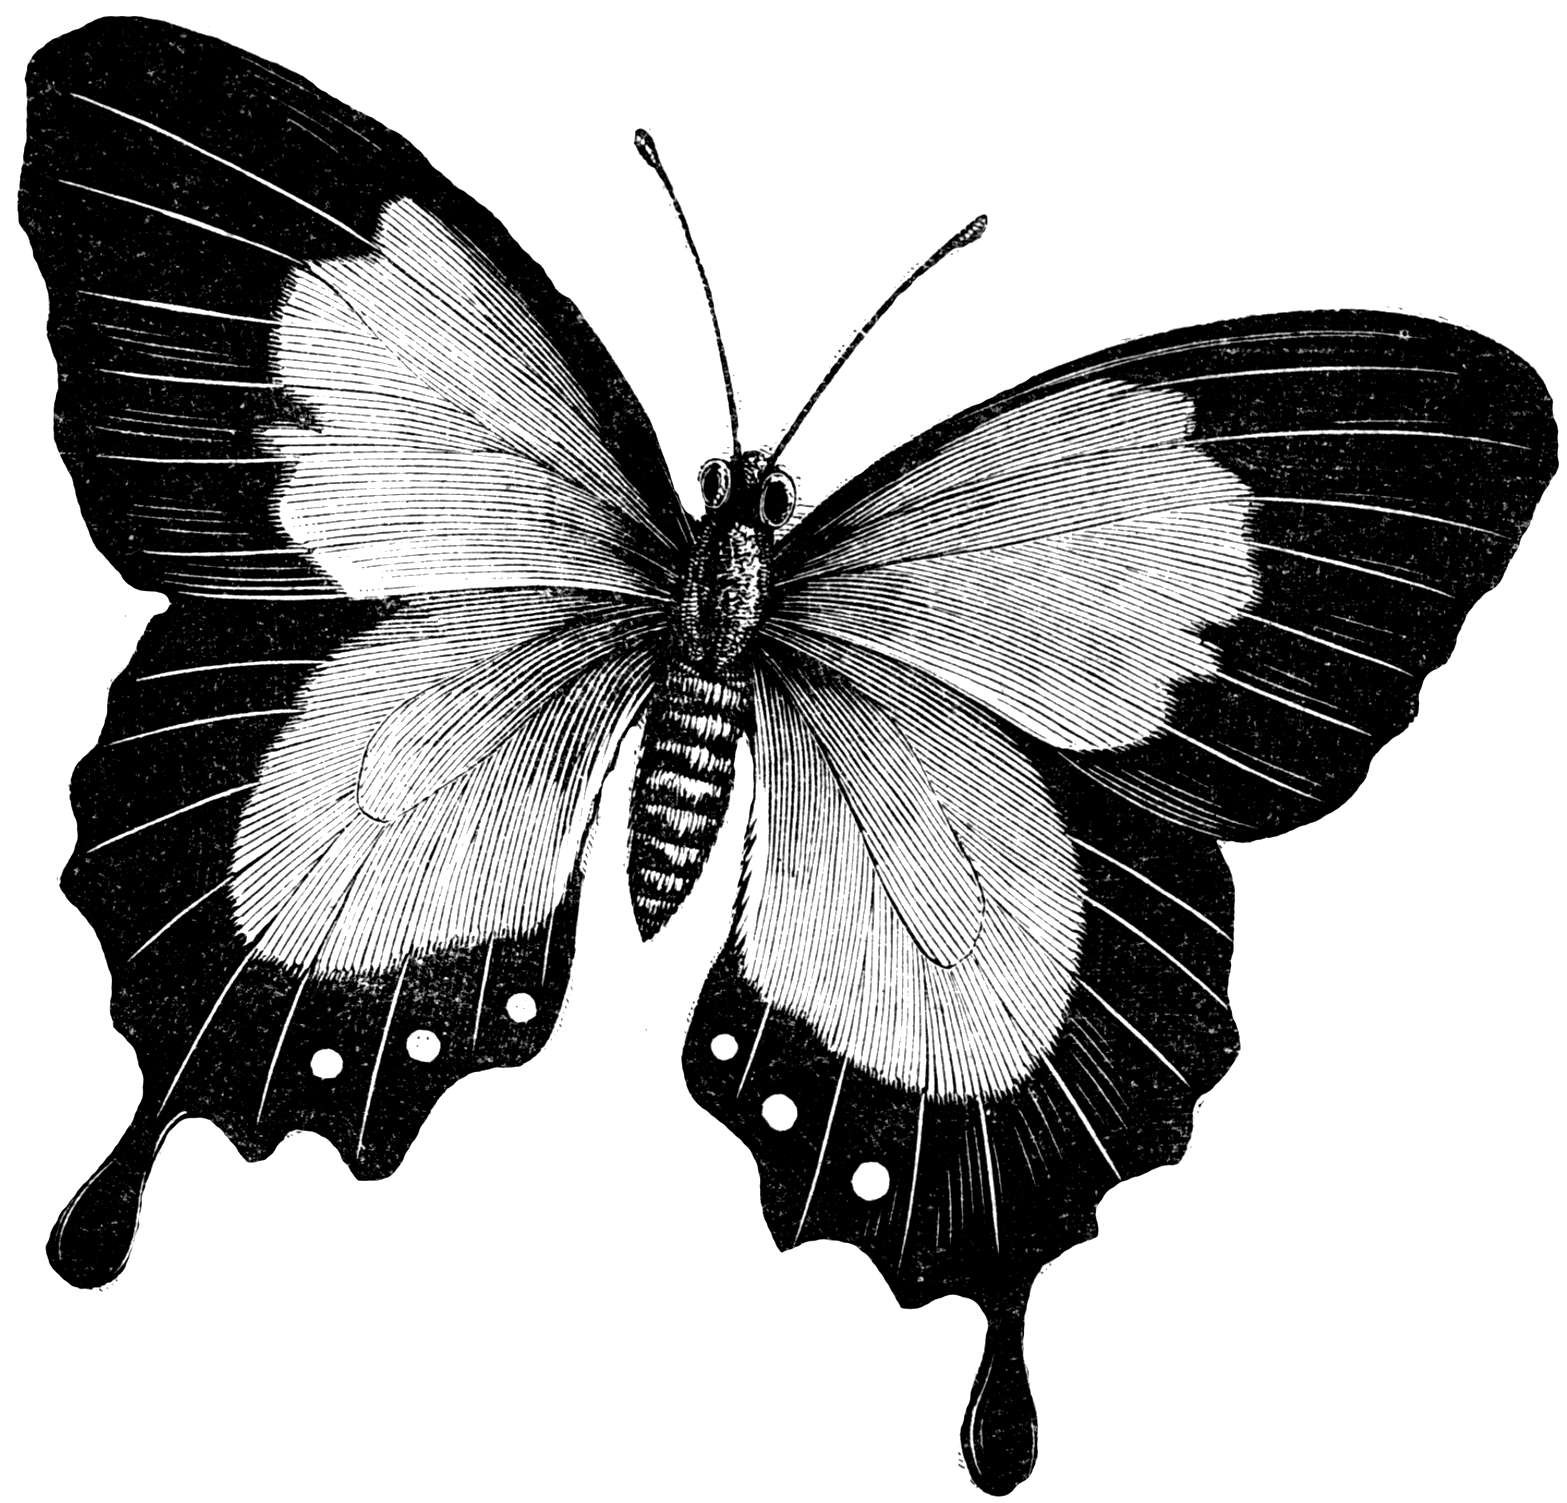
\includegraphics[width=1.5\textwidth]{butterfly_2_lg.png}};
               % from https://etc.usf.edu/clipart/3100/3126/butterfly_2.htm
      \end{tikzpicture}};

%\node [shift={(-5cm,-5cm)}] at (current page.north east) % Revision 2
%      {\begin{tikzpicture}[remember picture, overlay]
%          \draw[fill=black] (0,5) -- (1.5,5) -- (5,1.5) -- (5,0) -- cycle ;
%          \node[inner sep=0pt,rotate=-45] (rev) at (2.9,2.9) {\huge\color{white}\textbf{Revision 2}};
%      \end{tikzpicture}};

\node [align=center] at (current page.south) % bottom
      {\begin{tikzpicture}[remember picture, overlay]
          \node[anchor=south west, align=left] at (-10,0.5)
               {\resizebox{1\linewidth}{!}
                 {\Huge\color{black}
                   \textbf{Prototype\color{blue!30}'\color{black}Engineering
                   	Studio\textsuperscript{\large{\textregistered}}}}};      
                    % Studio\textsuperscript{\large{\textregistered}}}}};
               \node[anchor=south east, align=right] at (10,0.5) {\Huge\color{black}\textbf{Technicus}};
      \end{tikzpicture}};

\end{tikzpicture}

\end{document}
